\subsection{Creación de Cuenta Contable}

\begin{enumerate}

\item
    \begin{minipage}[t]{\linewidth}
        Ingresar a  \url{https://mdm.somoscmi.com:8443/ebx-ui/ui/custom/Cuentas/action/305}
        \raggedright
        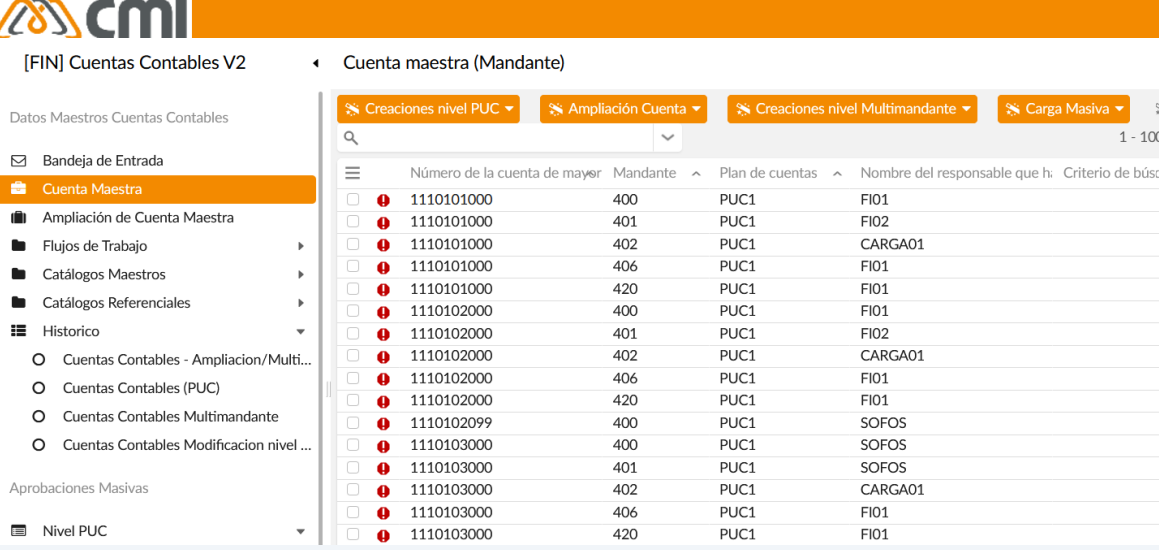
\includegraphics[width=0.8\textwidth]{NivelPUC/Creacion/ImgCreacion/CS01.png}

    \end{minipage}

\item
    \begin{minipage}[t]{\linewidth}
       Dentro de "Cuenta maestra" se ubica el servicio de creación de cuenta a nivel PUC. \raggedright
        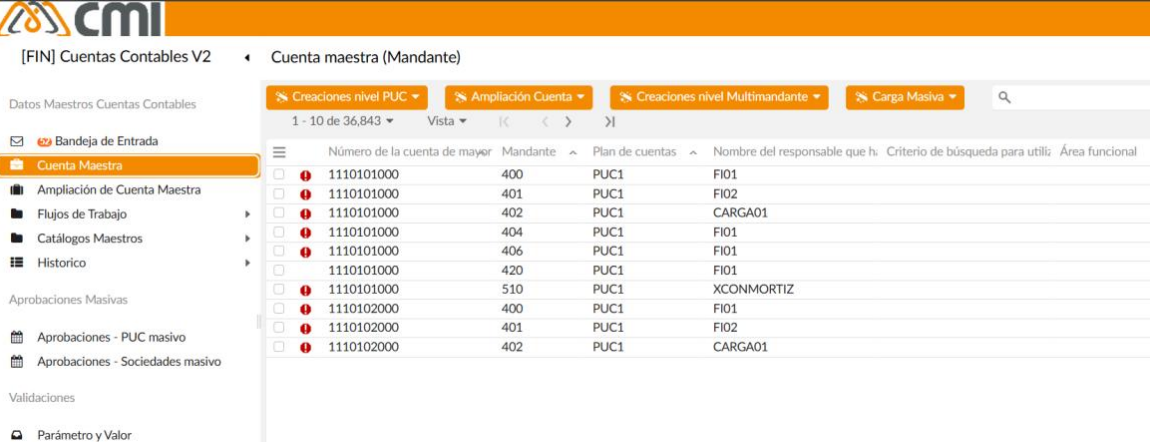
\includegraphics[width=0.8\textwidth]{NivelPUC/Creacion/ImgCreacion/CS02.png}

    \end{minipage}

\item
    \begin{minipage}[t]{\linewidth}
        Para iniciar una creación a nivel PUC se da click en "Creación Cuenta"

        \raggedright
        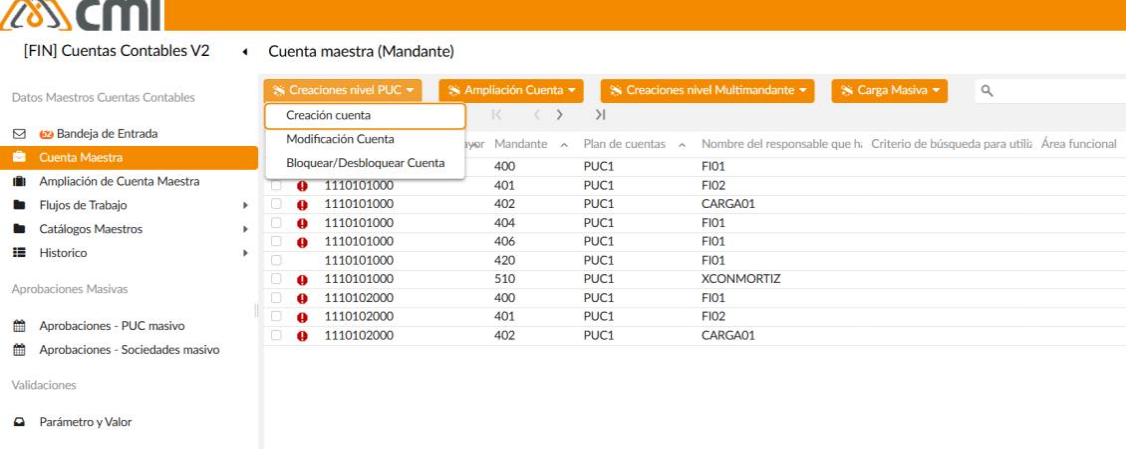
\includegraphics[width=0.8\textwidth]{NivelPUC/Creacion/ImgCreacion/CS03.png}

    \end{minipage}

\item
    \begin{minipage}[t]{\linewidth}
        Lo cual despliega un mensaje de confirmación para iniciar la creación de una cuenta.
        \raggedright
        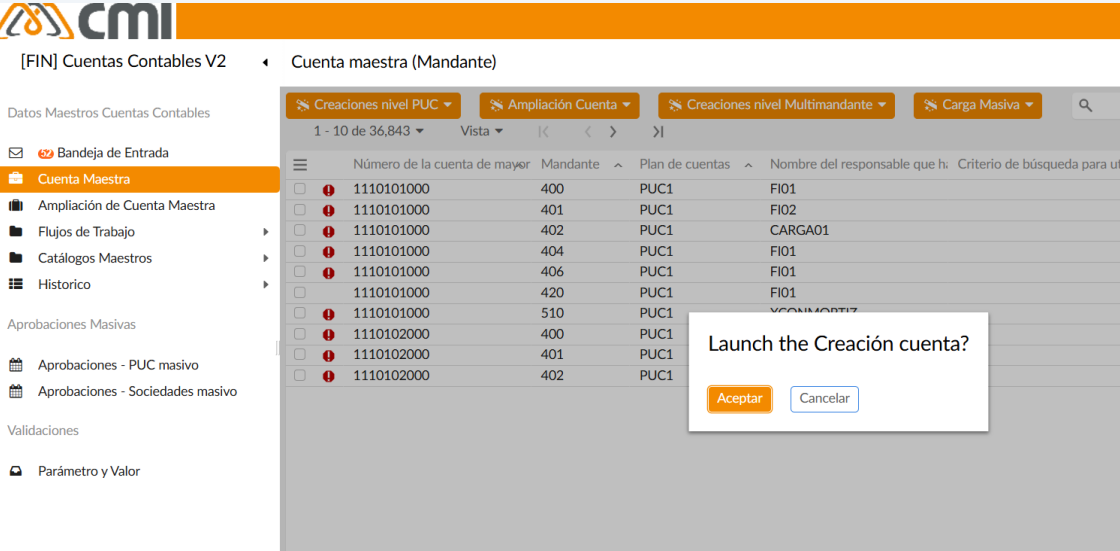
\includegraphics[width=0.8\textwidth]{NivelPUC/Creacion/ImgCreacion/CS04.png}

    \end{minipage}

\item
    \begin{minipage}[t]{\linewidth}
        Se despliega una pantalla donde se llevará a cabo el proceso de creación.

        \raggedright
        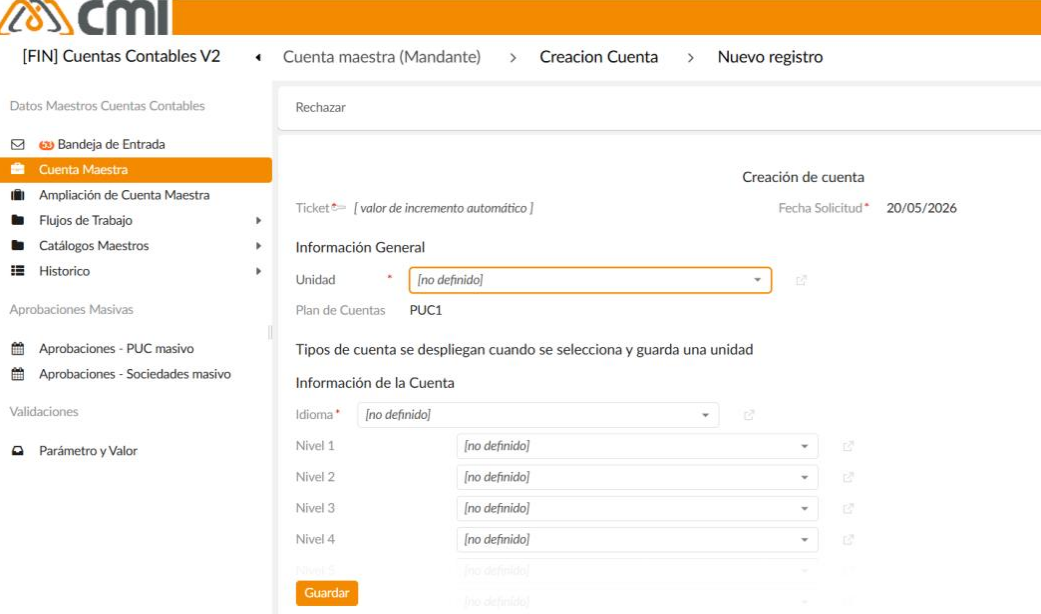
\includegraphics[width=0.8\textwidth]{NivelPUC/Creacion/ImgCreacion/CS05.png}

    \end{minipage}

\item
    \begin{minipage}[t]{\linewidth}
        001 - Vista del formulario de creación.

        \raggedright
        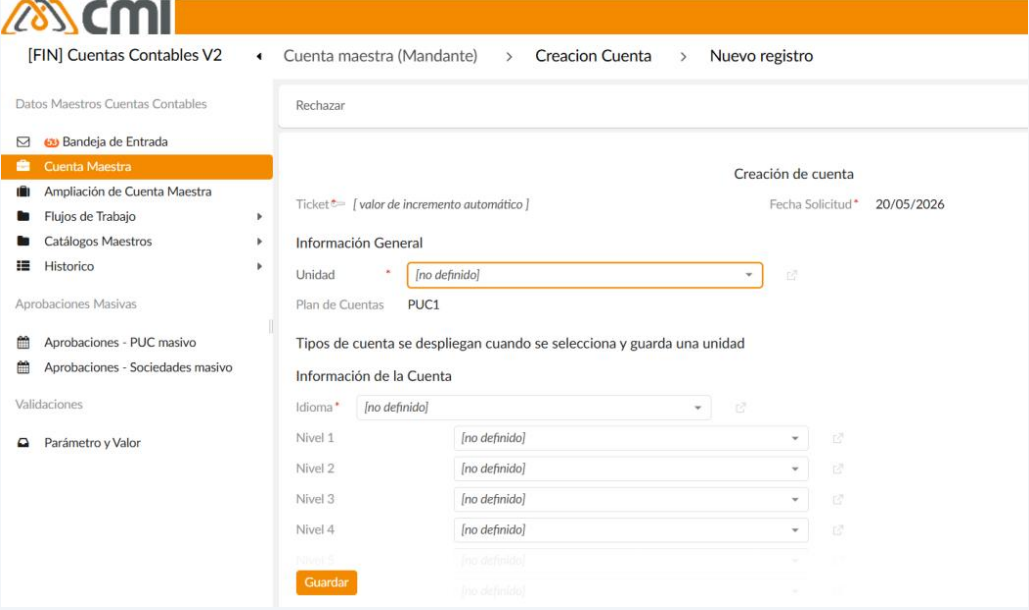
\includegraphics[width=0.8\textwidth]{NivelPUC/Creacion/ImgCreacion/CS06.png}

    \end{minipage}

\item
    \begin{minipage}[t]{\linewidth}
        Dentro el formulario se selecciona una unidad y al guardar aparece el tipo de cuenta a crear:

        \raggedright
        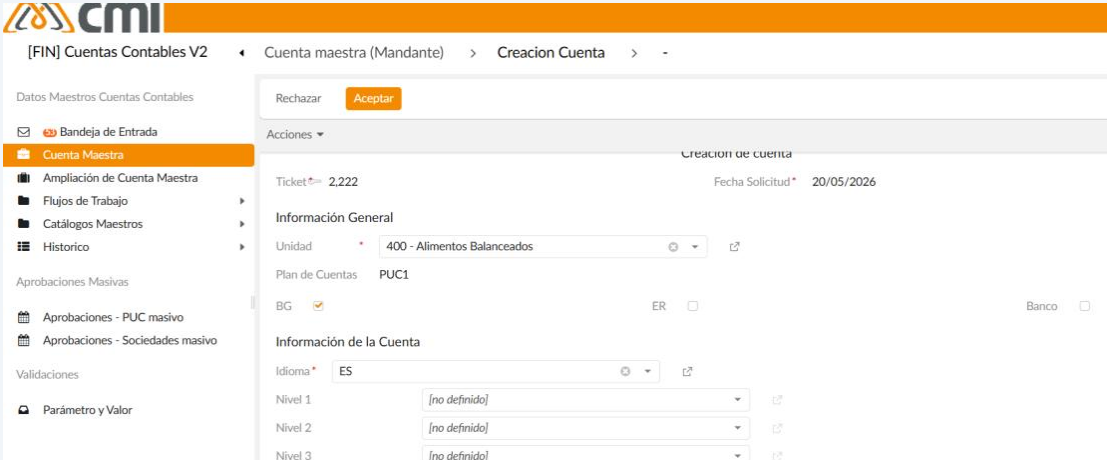
\includegraphics[width=0.8\textwidth]{NivelPUC/Creacion/ImgCreacion/CS07.png}

    \end{minipage}

\item
    \begin{minipage}[t]{\linewidth}
        \begin{itemize}
            \item BG: Balance General 
            \item ER: Estado de Resultados 
            \item Banco
        \end{itemize}
        
        \raggedright
        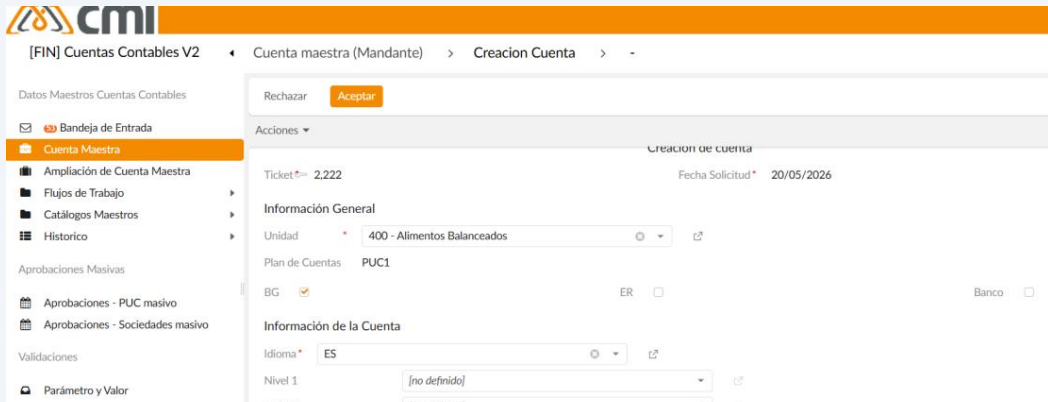
\includegraphics[width=0.8\textwidth]{NivelPUC/Creacion/ImgCreacion/CS08.png}

    \end{minipage}

\item
    \begin{minipage}[t]{\linewidth}
        Dentro el campo de unidad esta la lista de los mandantes y unidades disponibles.

        \raggedright
        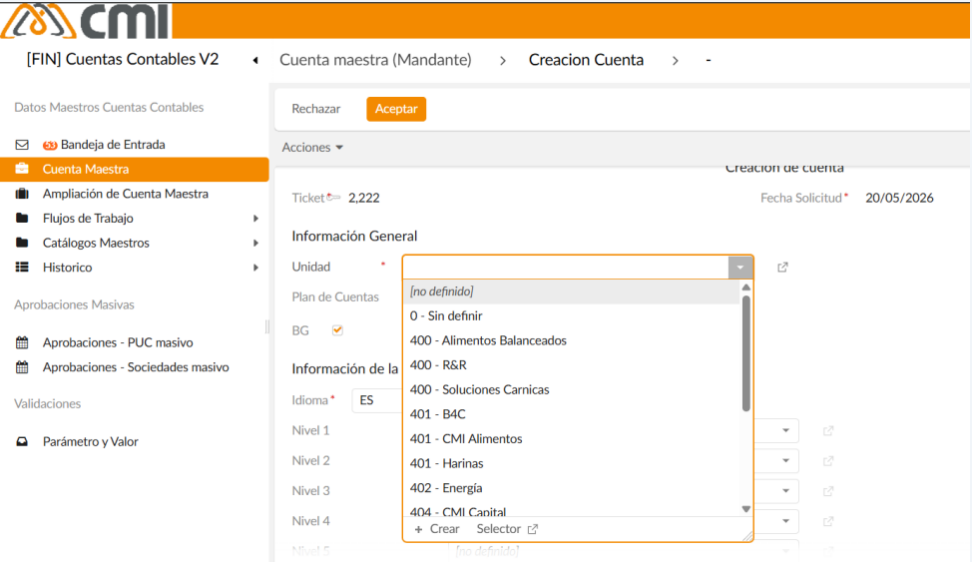
\includegraphics[width=0.8\textwidth]{NivelPUC/Creacion/ImgCreacion/CS09.png}

    \end{minipage}

\item
    \begin{minipage}[t]{\linewidth}
        Como siguiente paso se elige el tipo de idioma de la cuenta contable.

        \raggedright
        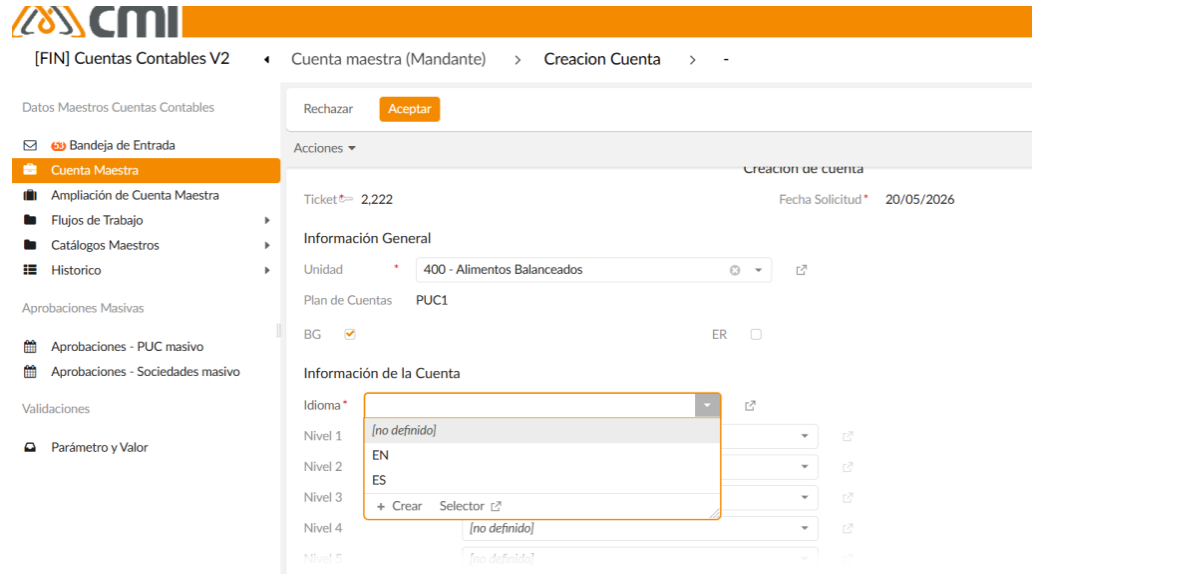
\includegraphics[width=0.8\textwidth]{NivelPUC/Creacion/ImgCreacion/CS10.png}

    \end{minipage}

\item
    \begin{minipage}[t]{\linewidth}
        En consiguiente se seleccionarán los niveles correctos para crear la cuenta contable.

        \raggedright
        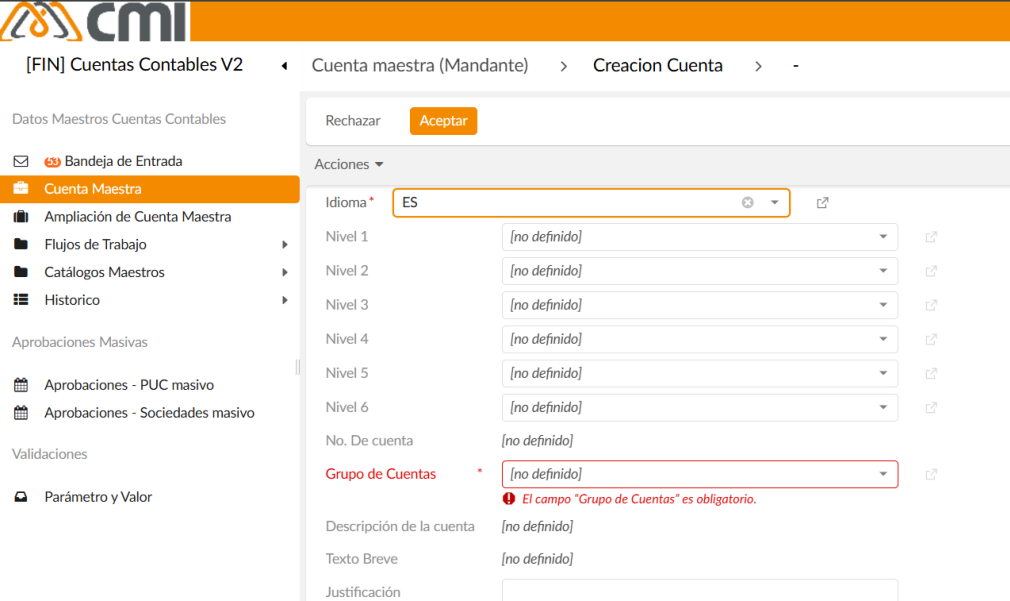
\includegraphics[width=0.8\textwidth]{NivelPUC/Creacion/ImgCreacion/CS11.png}

    \end{minipage}

\item
    \begin{minipage}[t]{\linewidth}
       Dentro el catálogo de "Nivel 1" se elige la opción correspondiente.

        \raggedright
        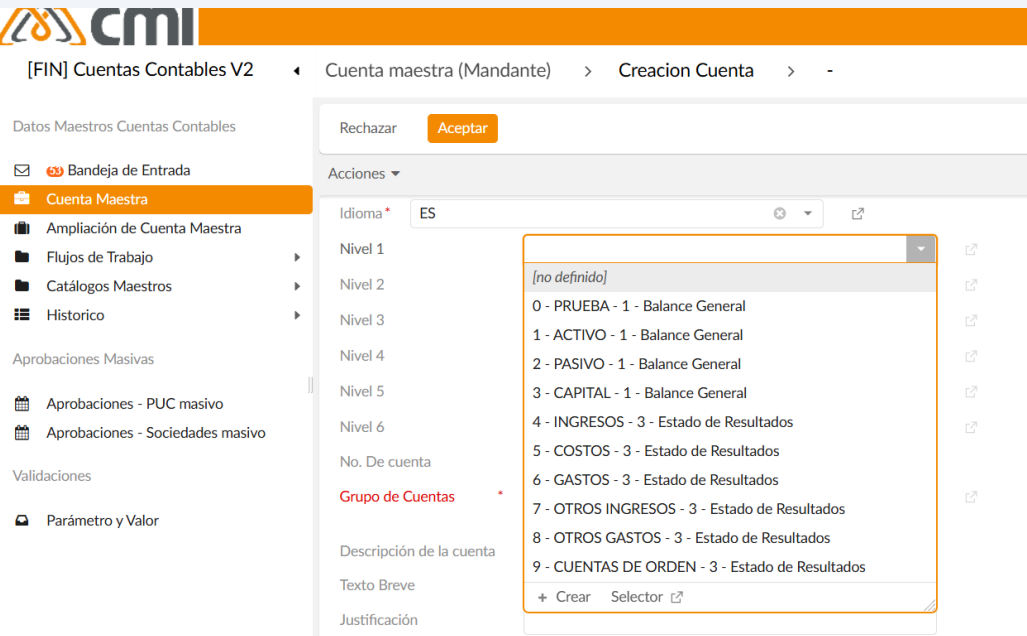
\includegraphics[width=0.8\textwidth]{NivelPUC/Creacion/ImgCreacion/CS12.png}

    \end{minipage}

\item
    \begin{minipage}[t]{\linewidth}
        Dentro el catálogo de "Nivel 2" se elige la opción correspondiente.

        \raggedright
        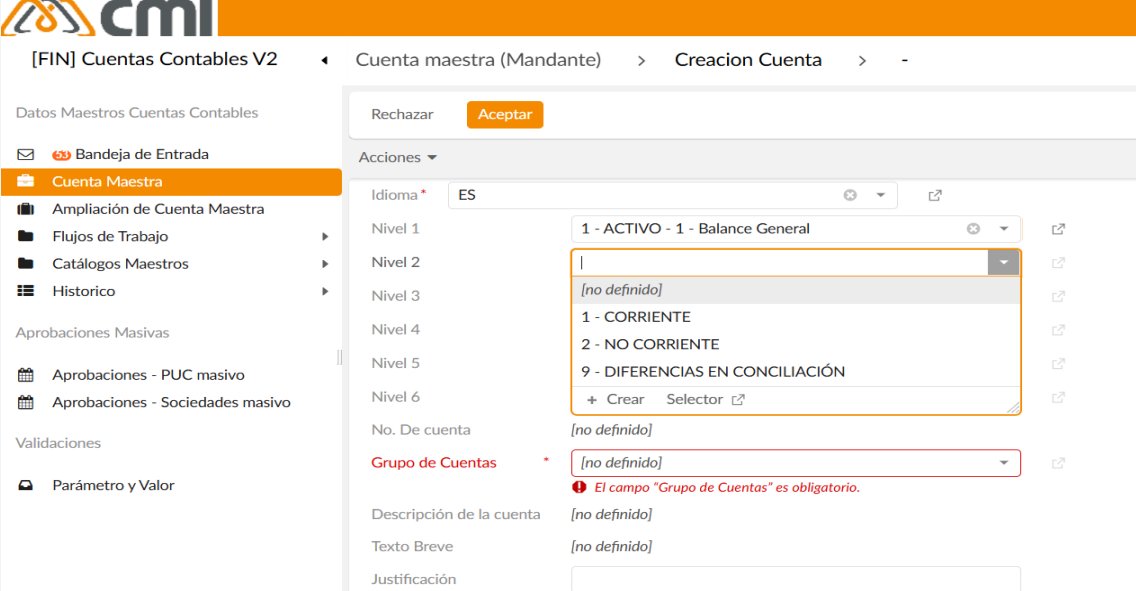
\includegraphics[width=0.8\textwidth]{NivelPUC/Creacion/ImgCreacion/CS13.png}

    \end{minipage}

\item
    \begin{minipage}[t]{\linewidth}
        Dentro el catálogo de "Nivel 3" se elige la opción correspondiente.

        \raggedright
        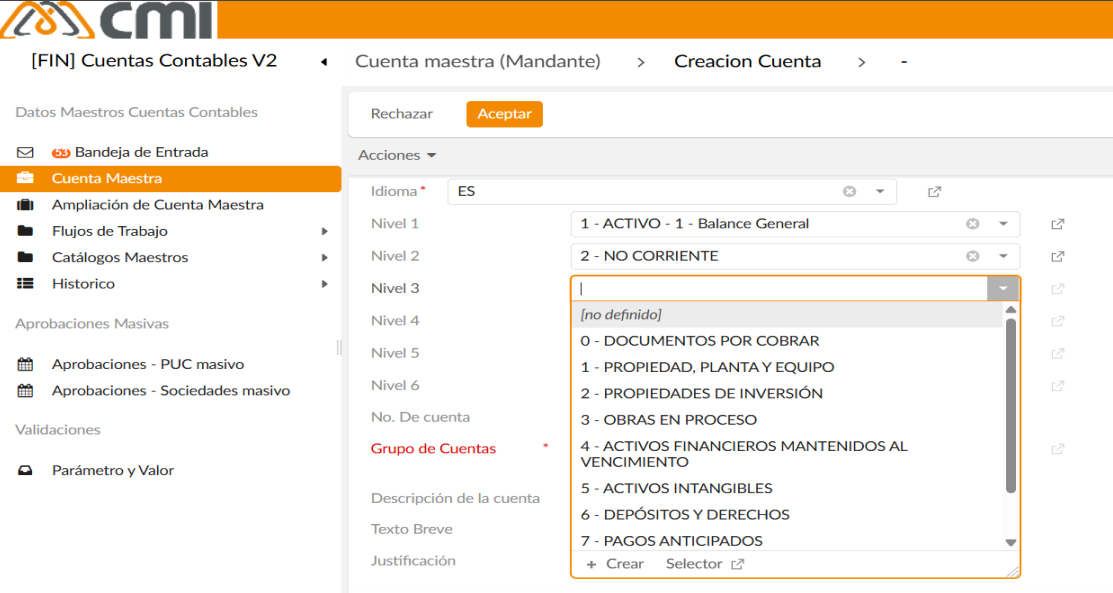
\includegraphics[width=0.8\textwidth]{NivelPUC/Creacion/ImgCreacion/CS14.png}

    \end{minipage}

\item
    \begin{minipage}[t]{\linewidth}
        Dentro el catálogo de "Nivel 4" se elige la opción correspondiente.
        
        \raggedright
        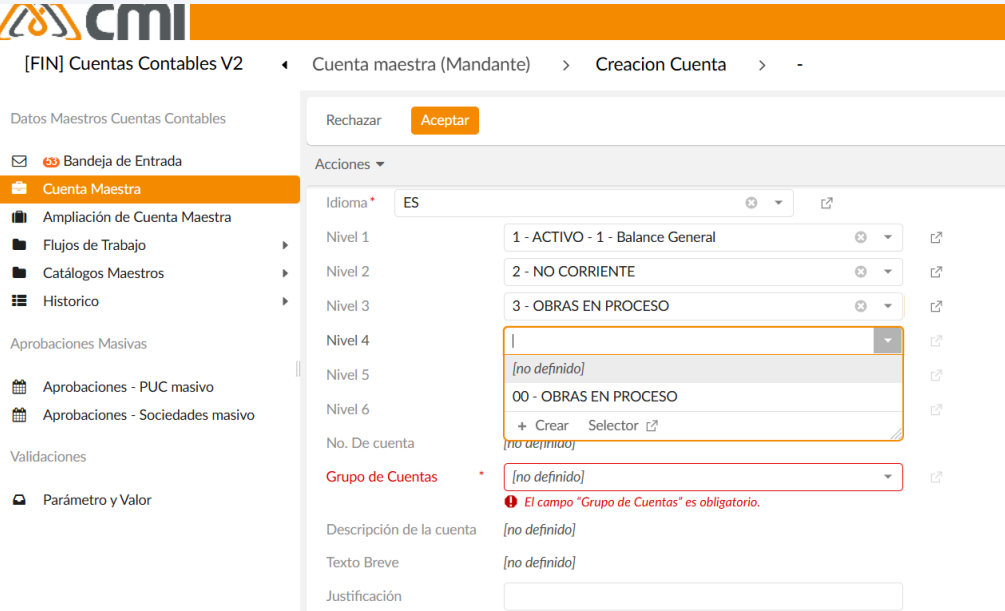
\includegraphics[width=0.8\textwidth]{NivelPUC/Creacion/ImgCreacion/CS15.png}

    \end{minipage}

\item
    \begin{minipage}[t]{\linewidth}
        Dentro el catálogo de "Nivel 5" se elige la opción correspondiente.

        \raggedright
        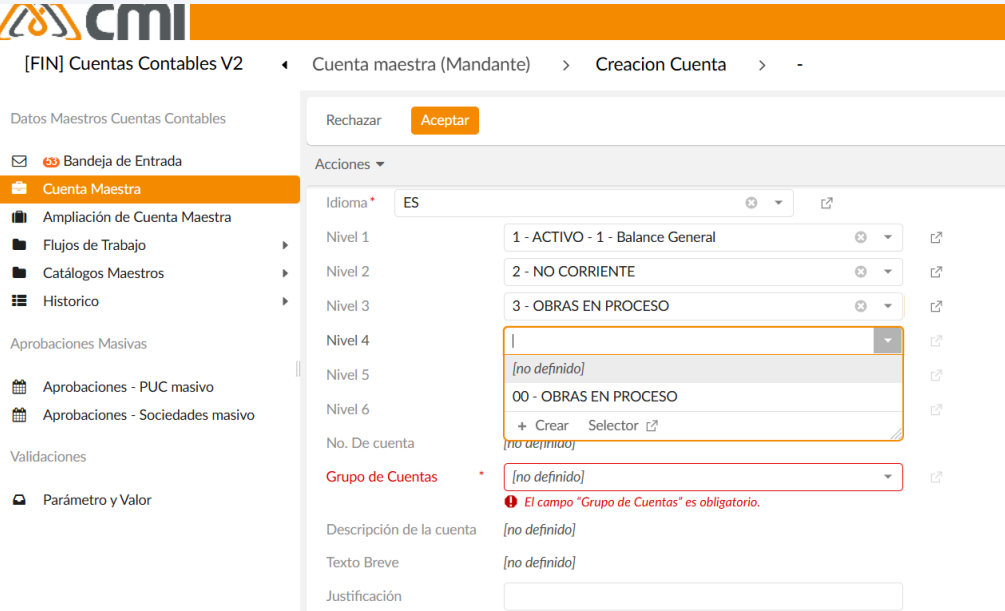
\includegraphics[width=0.8\textwidth]{NivelPUC/Creacion/ImgCreacion/CS15.png}

    \end{minipage}

\item
    \begin{minipage}[t]{\linewidth}
        Dentro el catálogo de "Nivel 6" se elige la opción correspondiente.

        \raggedright
        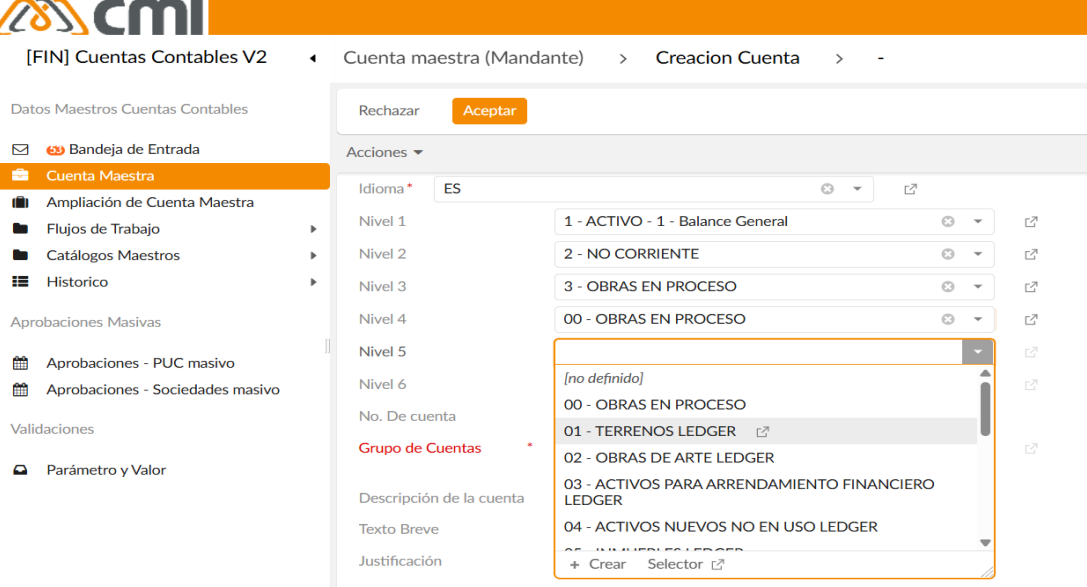
\includegraphics[width=0.8\textwidth]{NivelPUC/Creacion/ImgCreacion/CS16.png}

    \end{minipage}

\end{enumerate}

